\begin{savequote}[75mm]
The imagination of nature is far, far greater than the imagination of man.
\qauthor{Richard Feynman}
\end{savequote}

\chapter{Observation of Vector Boson Fusion production of $H\rightarrow WW^{*}\rightarrow \ell\nu\ell\nu$}

\section{Introduction}

After the discovery of a particle consistent with the Higgs boson, the $\HWW$ analysis had two main goals. The first goal was to increase the sensitivity of the analysis to fully confirm that the $\HWW$ process did indeed exist. The second goal was to characterize the particle as much as possible, including searching for the lower cross-section production modes, in order to confirm that it was indeed a Higgs boson.   This chapter presents a dedicated search for Vector Boson Fusion (VBF) production of a Higgs boson decaying via the \HWWfull mode. First, basics of the topology of VBF production are presented. Then, the details of the analysis are shown, including signal region definition, background estimation techniques, and systematic uncertainties. Finally, the results of the analysis are shown. As will be shown, this analysis is the first and most sensitive observation of the VBF production mode of the Higgs on ATLAS.

\section{Topology of VBF $\HWW$ production}

As discussed in Chapter 1, the characteristic feature of VBF production of the Higgs is the presence of two additional forward jets coming from the incoming partons which radiate the vector bosons that make the Higgs. These jets are forward because the outgoing partons still carry the longitudinal momentum of the incoming partons. Figure~\ref{fig:VBF_LeadJetEta} shows the distribution of the $\eta$ for the leading jet in a VBF event compared to a background top pair production event. As can be seen, the VBF jets tend to be more forward in $\eta$, while the $\ttbar$ jets are more central. 

\begin{figure}
  \vspace{20pt}
  \centering
  \hspace*{-32pt}
  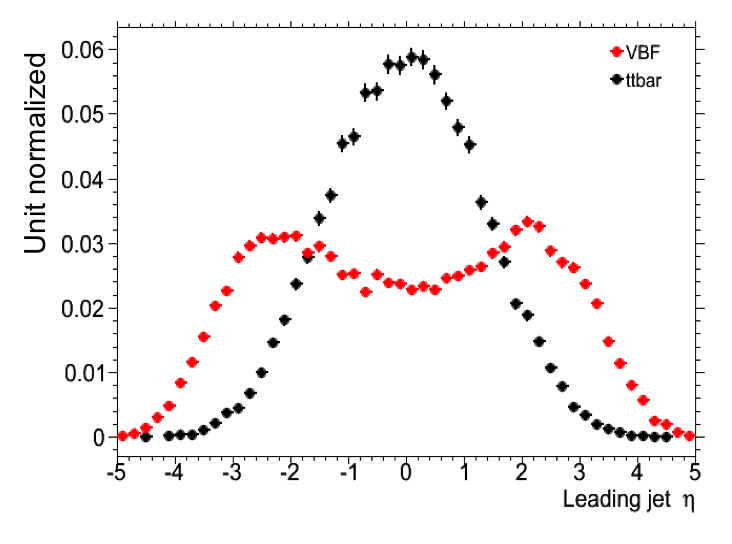
\includegraphics[width=0.6\textwidth]{figures/VBF_LeadJetEta}
  \caption{Leading jet $\eta$ in VBF $\HWW$ (red) and $\ttbar$ (black)}
  \label{fig:VBF_LeadJetEta}
\end{figure}

Because the cross section for VBF production is about an order of magnitude smaller than gluon fusion production, these forward jets must be used in order to better reduce background and achieve a good signal to background ratio. The analysis selection is constructed to maximally exploit the features of the unique VBF topology. 

\section{Data and simulation samples}

The results presented here are with 20.3 \ifb taken at $\sqrt{s} = 8 \TeV$ and 4.5 \ifb taken at $\sqrt{s} = 7 \TeV$. The details of the LHC and detector conditions during this period are given in Chapter 2. The trigger selection defining the dataset is discussed in section~\ref{sec:HWWtrigger}. The simulation samples used for signal and background modeling are given in section~\ref{sec:HWWMC}.

\subsection{Triggers}
\label{sec:HWWtrigger}

The analysis uses a combination of single lepton and dilepton triggers to allow lowering of the $\pT$ thresholds and increased signal acceptance. As discussed in Chapter 2, there are multiple levels in the ATLAS trigger system, and there are different $\pT$ thresholds imposed for the leptons at each level. Additionally, some triggers have a loose selection on the isolation of the lepton (looser than that applied offline in the analysis object selection). Table~\ref{tab:single-lepton-trig} shows the thresholds used for single lepton triggers, while table~\ref{tab:dilepton-trig} shows the thresholds coming from di-lepton triggers. The single lepton trigger efficiency for muons that pass the analysis object selection is 70\% for muons in the barrel region ($|\eta| < 1.05$) and 90\% in the endcap region. The electron trigger efficiency increases with electron $\pT$ but the average is approximately 90\%. These efficiencies are measured by combined performance and trigger signature groups\cite{ElectronTrigger2012,MuonTrigger2012}.



\begin{table}[h!]
\centering
\captionsetup{justification=centering}

%\begin{tabular*}{0.480\textwidth}{p{0.075\textwidth} p{0.180\textwidth} l}
\hspace{-10pt}
\begin{tabular}{|c|c|c|}
\hline
 & Level-1 threshold & High-level threshold \\ \hline \hline
\multirow{2}{*}{Electron} & $18$ & $24i$ \\ 
 & $30$ & $60$ \\ \hline

\multirow{2}{*}{Muon} & \multirow{2}{*}{$15$} & $24i$ \\ 
& & $36$ \\ 
 \hline

\end{tabular}

\caption{
Single lepton triggers used for electrons and muons. A logical ``or" of the triggers listed for each lepton type is taken. Units are in GeV, and the $i$ denotes an isolation requirement in the trigger. 
}
\label{tab:single-lepton-trig}
\end{table}

\begin{table}[h!]
\centering
\captionsetup{justification=centering}

%\begin{tabular*}{0.480\textwidth}{p{0.075\textwidth} p{0.180\textwidth} l}
\hspace{-10pt}
\begin{tabular}{|c|c|c|}
\hline
 & Level-1 threshold & High-level threshold \\ \hline \hline
$ee$ & $10$ and $10$ & $12$ and $12$ \\ \hline
$\mu\mu$ & $15$ & $18$ and $8$ \\ \hline
$e\mu$ & $10$ and $6$ & $12$ and $8$ \\ \hline
\end{tabular}

\caption{
Di-lepton triggers used for different flavor combinations. The two thresholds listed refer to leading and sub-leading leptons, respectively. The di-muon trigger only requires a single lepton at level-1. 
}
\label{tab:dilepton-trig}
\end{table}

The combination of all triggers shown gives good efficiency for signal events. This efficiency is summarized in table~\ref{tab:trigeff}. The relative improvement in efficiency by adding the dilepton triggers is also shown in the same table. The largest gain comes in the $\mu\mu$ channel. Overall the trigger selection shows a good efficiency for $\HWW$ signal events.

\begin{table}[h!]
\centering
\captionsetup{justification=centering}

%\begin{tabular*}{0.480\textwidth}{p{0.075\textwidth} p{0.180\textwidth} l}
\hspace{-10pt}
\begin{tabular}{|c|c|c|}
\hline
Channel & Trigger efficiency & Gain from $2\ell$ trigger \\ \hline \hline
$ee$ & $97$\% & $9.1$\% \\ \hline
$\mu\mu$ & $89$\% & $18.5$\% \\ \hline
$e\mu$ & $95$\% & $8.3$\% \\ \hline
$\mu e$ & $81$\% & $8.2$\% \\ \hline


\end{tabular}

\caption{
Trigger efficiency for signal events and relative gain of adding a dilepton trigger on top of the single lepton trigger selection. The first lepton is the leading, while the second is the sub-leading. Efficiencies shown here are for the ggF signal in the $\Njet = 0$ category but are comparable for the VBF signal. 
}
\label{tab:trigeff}
\end{table}



\subsection{Monte Carlo samples}
\label{sec:HWWMC}

Modeling of signal and background processes in the signal region, in particular for the $\mTH$ distribution, is an important consideration for the final interpretation of the analysis. Therefore, careful consideration must be paid to 

\section{Object selection}

\section{Analysis selection}

\section{Background estimation}

\section{Systematic uncertainties}

\section{Results}
